\documentclass[10pt]{article}
\usepackage{icmlko}

\icmlmeta{IP 파운데이션 월드모델}{92}{도구는 쉰 건이면 다 배운다}{다섯 노트가 가리키던 팝업 표본 병목을 갈랐다 --- 제품은 이미 쓸 수 있고 못 하는 것은 연구다}

\begin{document}

\twocolumn[
\icmlheader

\begin{abstract}
노트 91이 도메인마다 좋은 성분 수가 다르다고 했다. 고르는 것이 값을 하는지
\textbf{반을 갈라} 검정했다 --- A반에서 $k$를 고르고 B반에서 잰다. \textbf{손해다}
($-$0.0130). 아이돌에서 A반이 $k{=}1$을 고르는데 B반에서 $-$0.187이다.
\textbf{선택은 잡음이고 $k{=}2$를 전역으로 유지한다.} 그리고 반을 가르다 보니
더 큰 것이 보였다 --- 도구 성적이 그 도메인에 쌓인 레코드 수에 어떻게 반응하는가.
\textbf{쉰 건이면 거의 포화한다.} 팝업은 20$\sim$75건에서 $+$0.24$\sim+$0.53으로
요동할 뿐 추세가 없고, 모바일은 800건에서 멈추며, \textbf{웹툰은 50건 $+$0.468에서
2,817건 $+$0.387로 오히려 내린다}. 이것이 지난 다섯 노트(75 · 86 · 87 · 90 · 91)가
``팝업 표본이 병목''이라 한 것을 갈라 준다. \textbf{팝업 표본은 도구 정확도의
병목이 아니다.} 병목인 것은 둘뿐이다 --- 설계 결정을 팝업 기준으로 판정하는 것
(510건, 노트 75)과 팝업 라벨을 모형에 쓰는 것(수백 건, 노트 86 · 87).
\textbf{제품은 이미 쓸 수 있고, 못 하는 것은 모형을 더 좋게 만드는 일이다.}
\end{abstract}
]

\begin{figure*}[t]
\centering
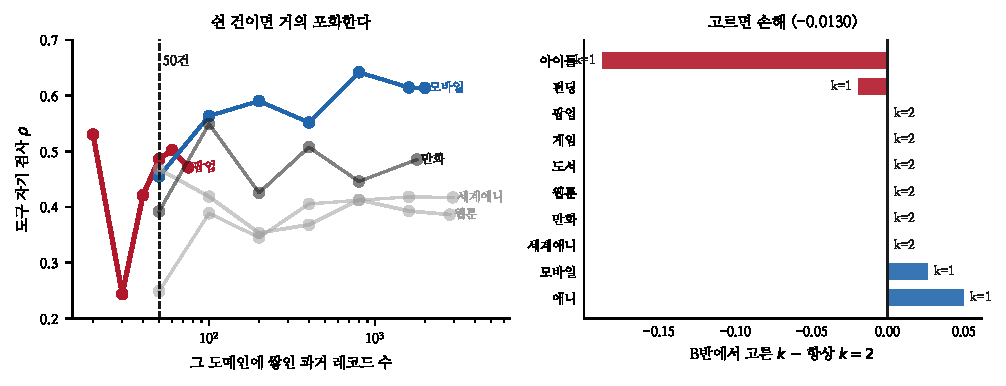
\includegraphics[width=\textwidth]{figs/hist.pdf}
\caption{왼쪽 --- 도구의 학습 곡선. 오른쪽 --- 성분 수 선택의 A/B 검정.}
\end{figure*}

\section{고르면 손해다}

\begin{table}[t]
\centering\tsize
\caption{A반에서 $k$를 고르고 B반에서 잰다.}
\begin{tabular}{lrrrr}
\toprule
& A반 고른 $k$ & B반 고른 것 & B반 $k{=}2$ & $\Delta$ \\
\midrule
애니 & 1 & $+$0.301 & $+$0.251 & $+$0.050 \\
모바일 & 1 & $+$0.655 & $+$0.629 & $+$0.026 \\
펀딩 & 1 & $+$0.280 & $+$0.299 & $-$0.019 \\
\textbf{아이돌} & 1 & $-$0.046 & $+$0.141 & \textbf{$-$0.187} \\
나머지 여섯 & 2 & --- & --- & $\pm$0.000 \\
\midrule
\textbf{평균} & & \textbf{$+$0.3272} & \textbf{$+$0.3402} & \textbf{$-$0.0130} \\
\bottomrule
\end{tabular}
\end{table}

\claimx{도메인별 성분 수 선택은 값을 안 한다 --- A반에서 고르고 B반에서 재면
$-$0.0130이다. 노트 91이 본 ``도메인마다 고르면 $+$0.3703''은 선택 편향이었다.}
{반을 한 번 갈랐다. 다른 분할이면 다를 수 있는데, 아이돌의 $-$0.187이 워낙
커서 부호가 바뀌기는 어렵다.}

노트 67(작은 표본 배선) · 80(부분집합) · 82(분모)에 이어 \textbf{같은 함정의
네 번째 사례}다. 이번에는 미리 갈라 놓고 걸렸다.

\section{도구는 쉰 건이면 다 배운다}

\begin{table}[t]
\centering\tsize
\caption{과거 레코드 수와 도구 자기 검사 $\rho$.}
\begin{tabular}{lrrrrr}
\toprule
& 50 & 100 & 400 & 800 & 전체 \\
\midrule
모바일 & $+$0.455 & $+$0.563 & $+$0.552 & $+$0.642 & $+$0.614 \\
만화 & $+$0.392 & $+$0.549 & $+$0.507 & $+$0.446 & $+$0.485 \\
\textbf{웹툰} & \textbf{$+$0.468} & $+$0.419 & $+$0.368 & $+$0.413 &
\textbf{$+$0.387} \\
세계애니 & $+$0.249 & $+$0.389 & $+$0.406 & $+$0.412 & $+$0.417 \\
\midrule
\multicolumn{6}{l}{팝업: 20건 $+$0.530 · 30건 $+$0.244 · 40건 $+$0.421} \\
\multicolumn{6}{l}{\hspace{2.4em}50건 $+$0.486 · 60건 $+$0.502 · 75건 $+$0.471} \\
\bottomrule
\end{tabular}
\end{table}

\claimx{도구의 성적은 그 도메인에 쌓인 과거 레코드 수에 거의 반응하지 않는다 ---
쉰 건이면 포화한다. 웹툰은 50건에서 2,817건으로 가며 오히려 $-$0.081 내린다.}
{50건 아래는 표본이 작아 자기 검사 자체가 몹시 흔들린다(팝업 30건 $+$0.244,
40건 $+$0.421). ``쉰 건이면 된다''는 그 위쪽이 평평하다는 뜻이지 쉰 건이
안전하다는 뜻이 아니다.}

\begin{quote}\fontsize{9.5}{11.5}\selectfont
\textbf{왜 안 늘어나는가.} 도구는 그 도메인의 과거로 \emph{인자 공간}만 만들고
예측은 아홉 출처에서 온다. 인자 공간은 축 넷다섯 개의 주성분이라 쉰 건이면
충분히 안정된다. \textbf{과거를 더 쌓아도 배울 것이 없다.}
\end{quote}

\section{병목을 갈랐다}

지난 다섯 노트가 모두 ``팝업 표본''을 가리켰다. 무엇의 병목인지 갈라야 한다.

\begin{table}[t]
\centering\tsize
\caption{팝업 표본이 사는 것과 안 사는 것.}
\begin{tabular}{lll}
\toprule
& 필요 & 근거 \\
\midrule
\textbf{도구 정확도} & \textbf{$\sim$50건} & 이 노트 \\
설계 판정 & $\sim$510건 & 노트 75 \\
라벨 활용 & 수백 건 & 노트 86 · 87 \\
배수 구간 & $\sim$1,650건 & 노트 75 \\
\bottomrule
\end{tabular}
\end{table}

\textbf{팝업 75건은 도구를 쓰기에 충분하다.} 모자란 것은 연구용이다 --- 설계
결정을 팝업 기준으로 판정하는 것, 팝업 라벨을 모형에 넣는 것, ``몇 명 올지''를
말하는 것.

\claimx{제품은 이미 쓸 수 있다. 팝업 표본이 병목인 것은 \emph{모형을 더 좋게
만드는 일}이지 \emph{모형을 쓰는 일}이 아니다.}{도구 정확도가 $\rho\approx+$0.47에
머문다는 것은 그대로다. 쉰 건이면 포화한다는 것은 ``더 쌓아도 안 좋아진다''는
뜻이므로, 좋게 만들려면 다른 길이 필요하다.}

\section{한계}

\begin{itemize}[leftmargin=1.1em,itemsep=0.15em]
\item 학습 곡선을 표본 추출 세 번의 평균으로 냈다. 구간을 안 붙였고, 작은
      크기에서 요동이 크다.
\item 웹툰이 내려가는 이유를 모른다. 큰 표본에서 오래된 작품이 섞여 들어오는
      구성 변화로 보이지만 확인 안 했다.
\item 성분 수 A/B 검정을 한 번의 분할로 했다.
\item ``쉰 건이면 포화''는 지금 아홉 출처가 있을 때다. 출처가 적으면 그 도메인의
      과거가 더 중요할 것이다.
\item 도구 정확도 $\rho\approx+$0.47이 라벨 천장(0.72$\sim$0.75, 노트 83)의
      3분의 2다. 남은 3분의 1을 어디서 얻을지는 여전히 모른다.
\end{itemize}

\section{다음}

\begin{enumerate}[leftmargin=1.3em,itemsep=0.15em]
\item \textbf{도구를 실제로 쓰게 만든다} --- 기획 단계에서 채우는 양식과
      출력 형식을 다듬는다. 표본이 병목이 아니라면 남은 것은 사용성이다.
\item 웹툰이 표본에 따라 내려가는 이유 --- 구성 변화인지 확인한다.
\item 출처 수와 과거 레코드 수의 교환 --- 출처가 적을 때 과거가 더 중요한가.
\item 천장까지 남은 3분의 1. 지금까지 닫힌 지렛대 목록(노트 76 · 80 · 82 ·
      83 · 85--88 · 90)을 다시 훑어 빠진 것을 찾는다.
\end{enumerate}

\vspace{0.6em}
\hrule height 0.3pt
\vspace{0.5em}
{\footnotesize
\textbf{참고문헌}\\[0.3em]
Cawley, G. C., Talbot, N. L. C. (2010). On over-fitting in model selection and
subsequent selection bias in performance evaluation. \emph{JMLR}, 11, 2079--2107.\\[0.15em]
Varoquaux, G. (2018). Cross-validation failure: small sample sizes lead to large
error bars. \emph{NeuroImage}, 180, 68--77.\\[0.15em]
Ilin, A., Raiko, T. (2010). Practical approaches to principal component analysis
in the presence of missing values. \emph{JMLR}, 11, 1957--2000.\\[0.15em]
Ben-David, S. et al. (2010). A theory of learning from different domains.
\emph{Machine Learning}, 79(1--2), 151--175.\\[0.15em]
Kish, L. (1965). \emph{Survey Sampling}. Wiley.
}

\end{document}
